% Metódy inžinierskej práce

\documentclass[10pt,oneside,slovak,a4paper]{article}

\usepackage[slovak]{babel}
%\usepackage[T1]{fontenc}
\usepackage[IL2]{fontenc} % lepšia sadzba písmena Ľ než v T1
\usepackage[utf8]{inputenc}
\usepackage{graphicx}
\usepackage{url} % príkaz \url na formátovanie URL
\usepackage{hyperref} % odkazy v texte budú aktívne (pri niektorých triedach dokumentov spôsobuje posun textu)
\usepackage{pdfpages}
\usepackage{cite}
%\usepackage{times}

\pagestyle{headings}

\title{Hry pre zdravie ako súčasť každodenného života\thanks{Semestrálny projekt v predmete Metódy inžinierskej práce, ak. rok 2022/23, vedenie: Ing.Igor Stupavský}} % meno a priezvisko vyučujúceho na cvičeniach

\author{Kristián Červenka\\[2pt]
	{\small Slovenská technická univerzita v Bratislave}\\
	{\small Fakulta informatiky a informačných technológií}\\
	{\small \texttt{xcervenkak@stuba.sk}}
	}

\date{\small 19. september 2022} % upravte



\begin{document}

\maketitle

\begin{abstract}
V tomto článku som sa preto rozhodol zamerať na vnášanie gamifikácie do oblasti zdravotníctva a využitie hier pre zdravie a ich vplyv v oblasti bežného života ľudí.
Objasním, čo sú to vlastne hry pre zdravie a ako vedia byť prospešné pre vývoj dieťaťa.
Ďalej by som sa chcel zamerať na zlepšenie životného štýlu používateľov hier pre to určených.Objasním hry pre zdravie na akom princípe fungujú a čo je zároveň ich cieľom.
Objasním princíp fungovania hier pre zdravie, ich cieľ a implementáciu v každodennom živote.
Spracujem tému ako sú hry jednou zo schopností ako prinútiť ľudí byť flexibilný , respektíve viacej sa hýbať v dnešnom technologickom svete a zároveň sa proaktívne vysporiadať s rýchlo meniacim svetom technológií. 
Hry sú jednou z možností ako zmeniť ľudské správanie na prijateľnejšie pre spoločnosť preto sa zameriam aj na hry pre psychické zdravie.
\end{abstract}



\section{Úvod}
Videohry ponúkajú inovatívne, vzrušujúce a vysoko efektívne metódy na zvyšovanie vedomostí a ovplyvňovanie zdravotných výsledkov. 
V 21.storočí rastie potreba chrániť zdravie ľudí prostredníctvom variácie dostupných zdrojov.
Jednou z možností ako zlepšiť zdravie ľudí pohybujúcich sa po tomto svete je zasadenie gamifikácie do prostredia zdravotníctva. 
Pre spracovanie témy som sa rozhodol z dôvodu nárastu dopytu hier hre zdravie.Videohry majú schopnosť zaujať používateľov inou cestou ako iné média.
V oblasti zdravotníctva sa videohry objavili v rôznych oblastiach. 
Za posledných dvadsať rokov sa používajú v odbornom výcviku, terapii, starostlivosti o seba, podpore zdravia i v komunikácii o zdraví.


\section{Motivácia} 
\subsection{Hry pre zdravie}
Videohry vo všeobecnosti majú schopnosť zaujať hráčov ako iným spôsobom ako ponúkajú dnešné novodobé média.Hry sa stávajú zaujímavou oblasťou rôznych výskumov a pokusov predvádzaných vedcami. Zo štúdie asociovanej Entertainment Software Association \cite{PLP-Framework} vyplýva , že približne 29\% hráčov sú v rozmedzí 18 a menej rokov. 
V súčastnosti využívame sofistikované technológie na podporu zdravia spôsobom , ktorý bol nepredstaviteľný pre minulé generácie.Množstvo hier pre zdravie je postavených na platformách dávno známych hráčom , ako sú napríklad osobné počítače alebo webové stránky.Hry podnecujú ich používateľov k opakovanému hraniu a preukazujú postupné  pozitívne zmeny správania potrebné na dosiahnutie individuálnych zdravotných zmien.
\subsection{Moderné pokroky v oblasti hier pre zdravie}
Vývoj a testovanie prebieha v širokom spektre chorôb , na prevenciu a liečbu zdravotných problémov.Bolo vykonaných množstvo výskumov zameraných na zdravotný stav človeka, akými sú napríklad cystická fibróza,liečba bolesti , Parkinsonova choroba , obezita a rôzne variácie vírusových ochorení.Tento výskum zahŕňal mimo iných i psychické  choroby a rehabilitácie, akými sú napríklad depresia, posttraumatická stresová porucha , úzkosť , popáleniny , mŕtvica,traumatické poškodenia mozgu a mnohé iné.Príkladom sú sociálne problémy , s ktorými sa ľudstvo stretáva takmer každý deň, násilie , šikanovanie , rasové predsudky\cite{bworld}.
\label{nejaka}
\section{Modifikácie hier pre zdravie v oblastiach bežného života}

\subsection{Hry ako forma edukácie prospešná pre vývoj dieťaťa}
Hry sú formou rekreácie, ktorá sa vo všeobecnosti považuje za prospešnú pre rozvoj dieťaťa. Vo väčšine prípadov majú hry pravidlá , ciele, možnosti voľby, výzvy a body , ktoré od mala nabádajú dieťa ku základným pravidlám spoločnosti. Príkladom sú seriózne hry , ktoré sú navrhnuté tak , aby mimo zábavy vniesli do života i iný účel.Tím vedcov zaoberajúcimi sa hrami o zdraví kategorizoval tieto hry do najmänej štyroch kategórií.Individálnou kategóriou hier pre zdravie sú hry určené na školenia zdravotníkov poskytujúcich zdravotnú starostlivosť. Herný dizajn ponúka mimo iného i prvky herného dizajnu , ktoré sú atraktívne pre rôzne vekové skupiny. Medzi základné prvky herného dizajnu patria napríklad interaktivita a spätná väzba. Pomocou nej majú možnosť hráči ihneď po inicializovaní akcie dostať okamžité informácie a ich dôsledok. Mimo iných majú hráči možnosť vyberať si identitu , pomocou ktorej získajú schopnosť stať sa hernou postavou a vytvoriť si vzťah a prepojenie s inými postavami v hre.
\paragraph{1.Hry pre zdravie na zvýšenie vedomostí.}

\paragraph{2.Hry pre zdravie spôsobujúce zmeny správania.}
\paragraph{3.Hry pre zdravie, ktoré zahŕňajú fyzickú aktivitu}
\paragraph{4.Hry pre zdravie ovplyvňujúce zdravotné prekurzory}
%\section{Modifikácie hier pre zdravie v oblastiach bežného života}
\paragraph{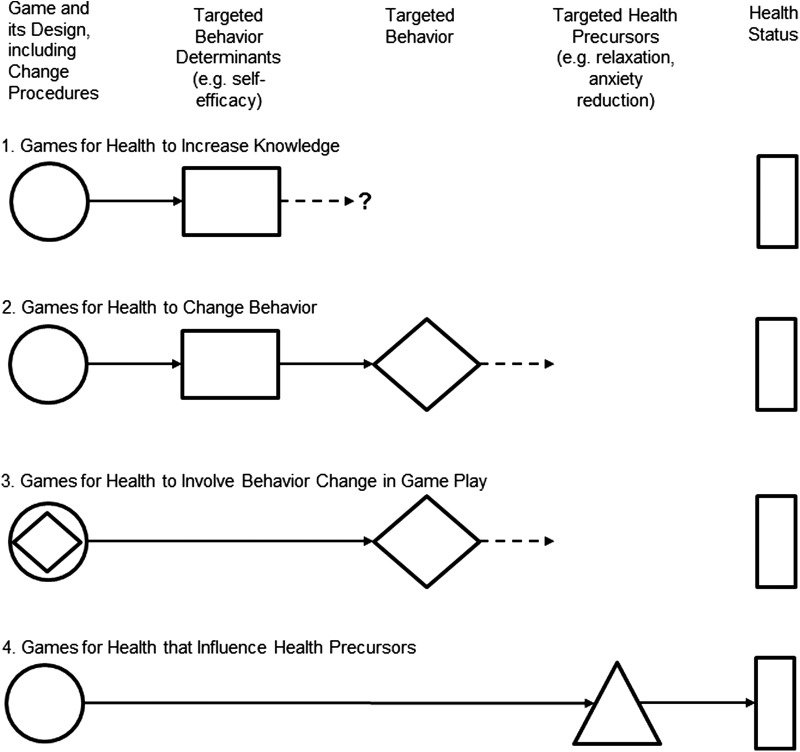
\includegraphics[scale=2]{tps_1.jpeg}}
\caption{1.obr Rozdelenie hier pre zdravie}

\subsection{1.Hry pre zdravie na zvýšenie vedomostí}
Mnohé zahraničné štúdie preukázali prepojenie zážitkových,herných, a vedomostných aspektov ako jednu z najlepších foriem učenia vôbec pre zapojenie študentov do akademických , zdravotných a spoločenských tématických oblastí.Zo štúdií vyplynulo , že hry ktoré ponúkajú možnosť učenia prostredníctvom ich hrania sú účinnejšie v metaanylýze 39 štúdií a umožňujú študentom lepšiu edukáciu ako tradičná výučba z hľadiska zapamätania si informácii z pohľadu študentov.Učitelia uvádzali , že vážne hry boli z hľadiska zapamätania informácií obzvlášť motivujúce pre študentov so slabými až mierne priemernými výsledkami,avšak toto samotné zvýšenie vedomostí nemusí viesť ku zlepšeniu zdravotného stavu.Napriek tomu , že herné výučbové technológie nie sú príliš rozširené, nedávny výskum ukázal , že až 55\% učiteľov využíva hry na skvalitnenie vzdelania svojich žiakov aspoň raz týždenne.Avšak medzi prvoradé prekážky využívania hier na edukáciu patrí najmä nedostatok času, vysoké náklady a nedostatok technologických prostriedkov v triedach.Dopomáhajú tomu i normy a požiadavky , ktoré vývojárom hier sťažujú DevOps hier určených na výučbu.

\subsection{2.Hry pre zdravie spôsobujúce zmeny správania}
Prvý vykonaný prieskum rôznych hier pre zdravie preukázal , že všetky okrem jedenj mali pozitívny vplyv na výsledky vzdelávania.Z výsledkov nedávnej metaanalýzy 64 hier propagujúcich zdravý životný štýl vyplýva, že všetky mali významný vplyv na spravanie a dokonca i na zdravotné výsledky ich používateľov.Príkladom boli videohry na vzdelávanie o cukrovke, ktoré mali pozivíny vplyv na vedomosti, zvládanie ochorenia a zlepšenie klinických výsledkov.Využitie virtuálnej reality a videohier na rehabilitáciu po úraze mozgu a hlavy zaznamenalo taktiež pozitívne výsledky v oblasti rovnováhy, funkcií horných končatín a rôznych testov kognitívnych funkcií. Z výsledkov štúdií dokonca vyplynulo , že využitie moderných metód liečby pomocou hier malo za následok  pozitívnejšie výsledky ako využitie tradičnej terapie.Systematický prehľad vykonaný šesťdesiatimi štyrmi štúdiami hier na terapeutické použitie odhalil sľubné výsledky zlepšenia zdravia pacientov a ich rehabiltáciu.Taktiež u pacientov trpiacich obezitov boli u viac ako 40\% zaznamenané pozitívne výsledky súvisiace s adipozitou.Mnohé štúdie teda potvrdzujú značnú účinnosť hier pri ovplyvňovaní vedomostí, spravania a zdravotných výsledkov.

\subsection{3.Hry pre zdravie, ktoré zahŕňajú fyzickú aktivitu}
Exergames sú hry, ktoré si vyžadujú na ich hranie a pokrok vykonávať fyzickú aktivitu.V posledných rokoch so stúpajúcim záujmom o zdravý životný štýl sa o tento typ hier prejavil značný záujem.Tanečné hry, ktoré sa najskôr vyskytovali iba v herniach sa pomocou snímačou hornej časti tela a podložky dolnej časti tela , ktoré zachytávajú pomocou AI pohyby končatín , začali vyskytovať i v bežných domácnostiach.Energetický výdaj pri týchto hrách bol značne vyšší ako pri hrách so sedavým charakterom.Začlenenie exergames do detských programov proti obezite preukázalo prínosy pre zníženie indexu telesnej hmotnosti ,zvýšenie fyzickej aktivity a zníženie času stráveného pri obrazovke.Deti vo veku od 6 do 11 rokov , ktoré hrali exergames pripojené ku stacionárnemu bicyklu, mali vyšší energetický výdaj ako deti , ktoré tieto hry nehrali.Mnohé výhody hier ako napríklad motivácia a zábava sa môžu kombinovať s pobytom vonku.V literatúre o exergames sa objavilo značné množstvo prehľadov. Niektoré z nich boli veľmi pozitívne a naznačovali , že tieto hry sú dôležitým nástrojom na prevenciu liečby obezity.Exergames častokrát vedú v domácich podmienkach k významným zmenám fyzickej aktivity, hmotnosti a kognitívnych funkcií.
\subsection{4.Hry pre zdravie ovplyvňujúce zdravotné prekurzory}
Hranie hier tesne pred operáciou znížilo úzkosti pacientov , čo súviselo s lepšími zdravotnými výsledami a skrátením dĺžky pobytu v nemocnici.Hranie mien bolo navrhnuté ako metóda na vyvolanie fyziologických zmien, ktoré môžu zvýšiť odolnosť , znížiť strach a úzkosť a zlepšiť zdravie pacientov s rakovinou.Interaktivita hier aktivovala oblasti mozgu , ktoré súviseli s pozitívnejším postojom k chemoterapii rakoviny.
\section{Diagram}
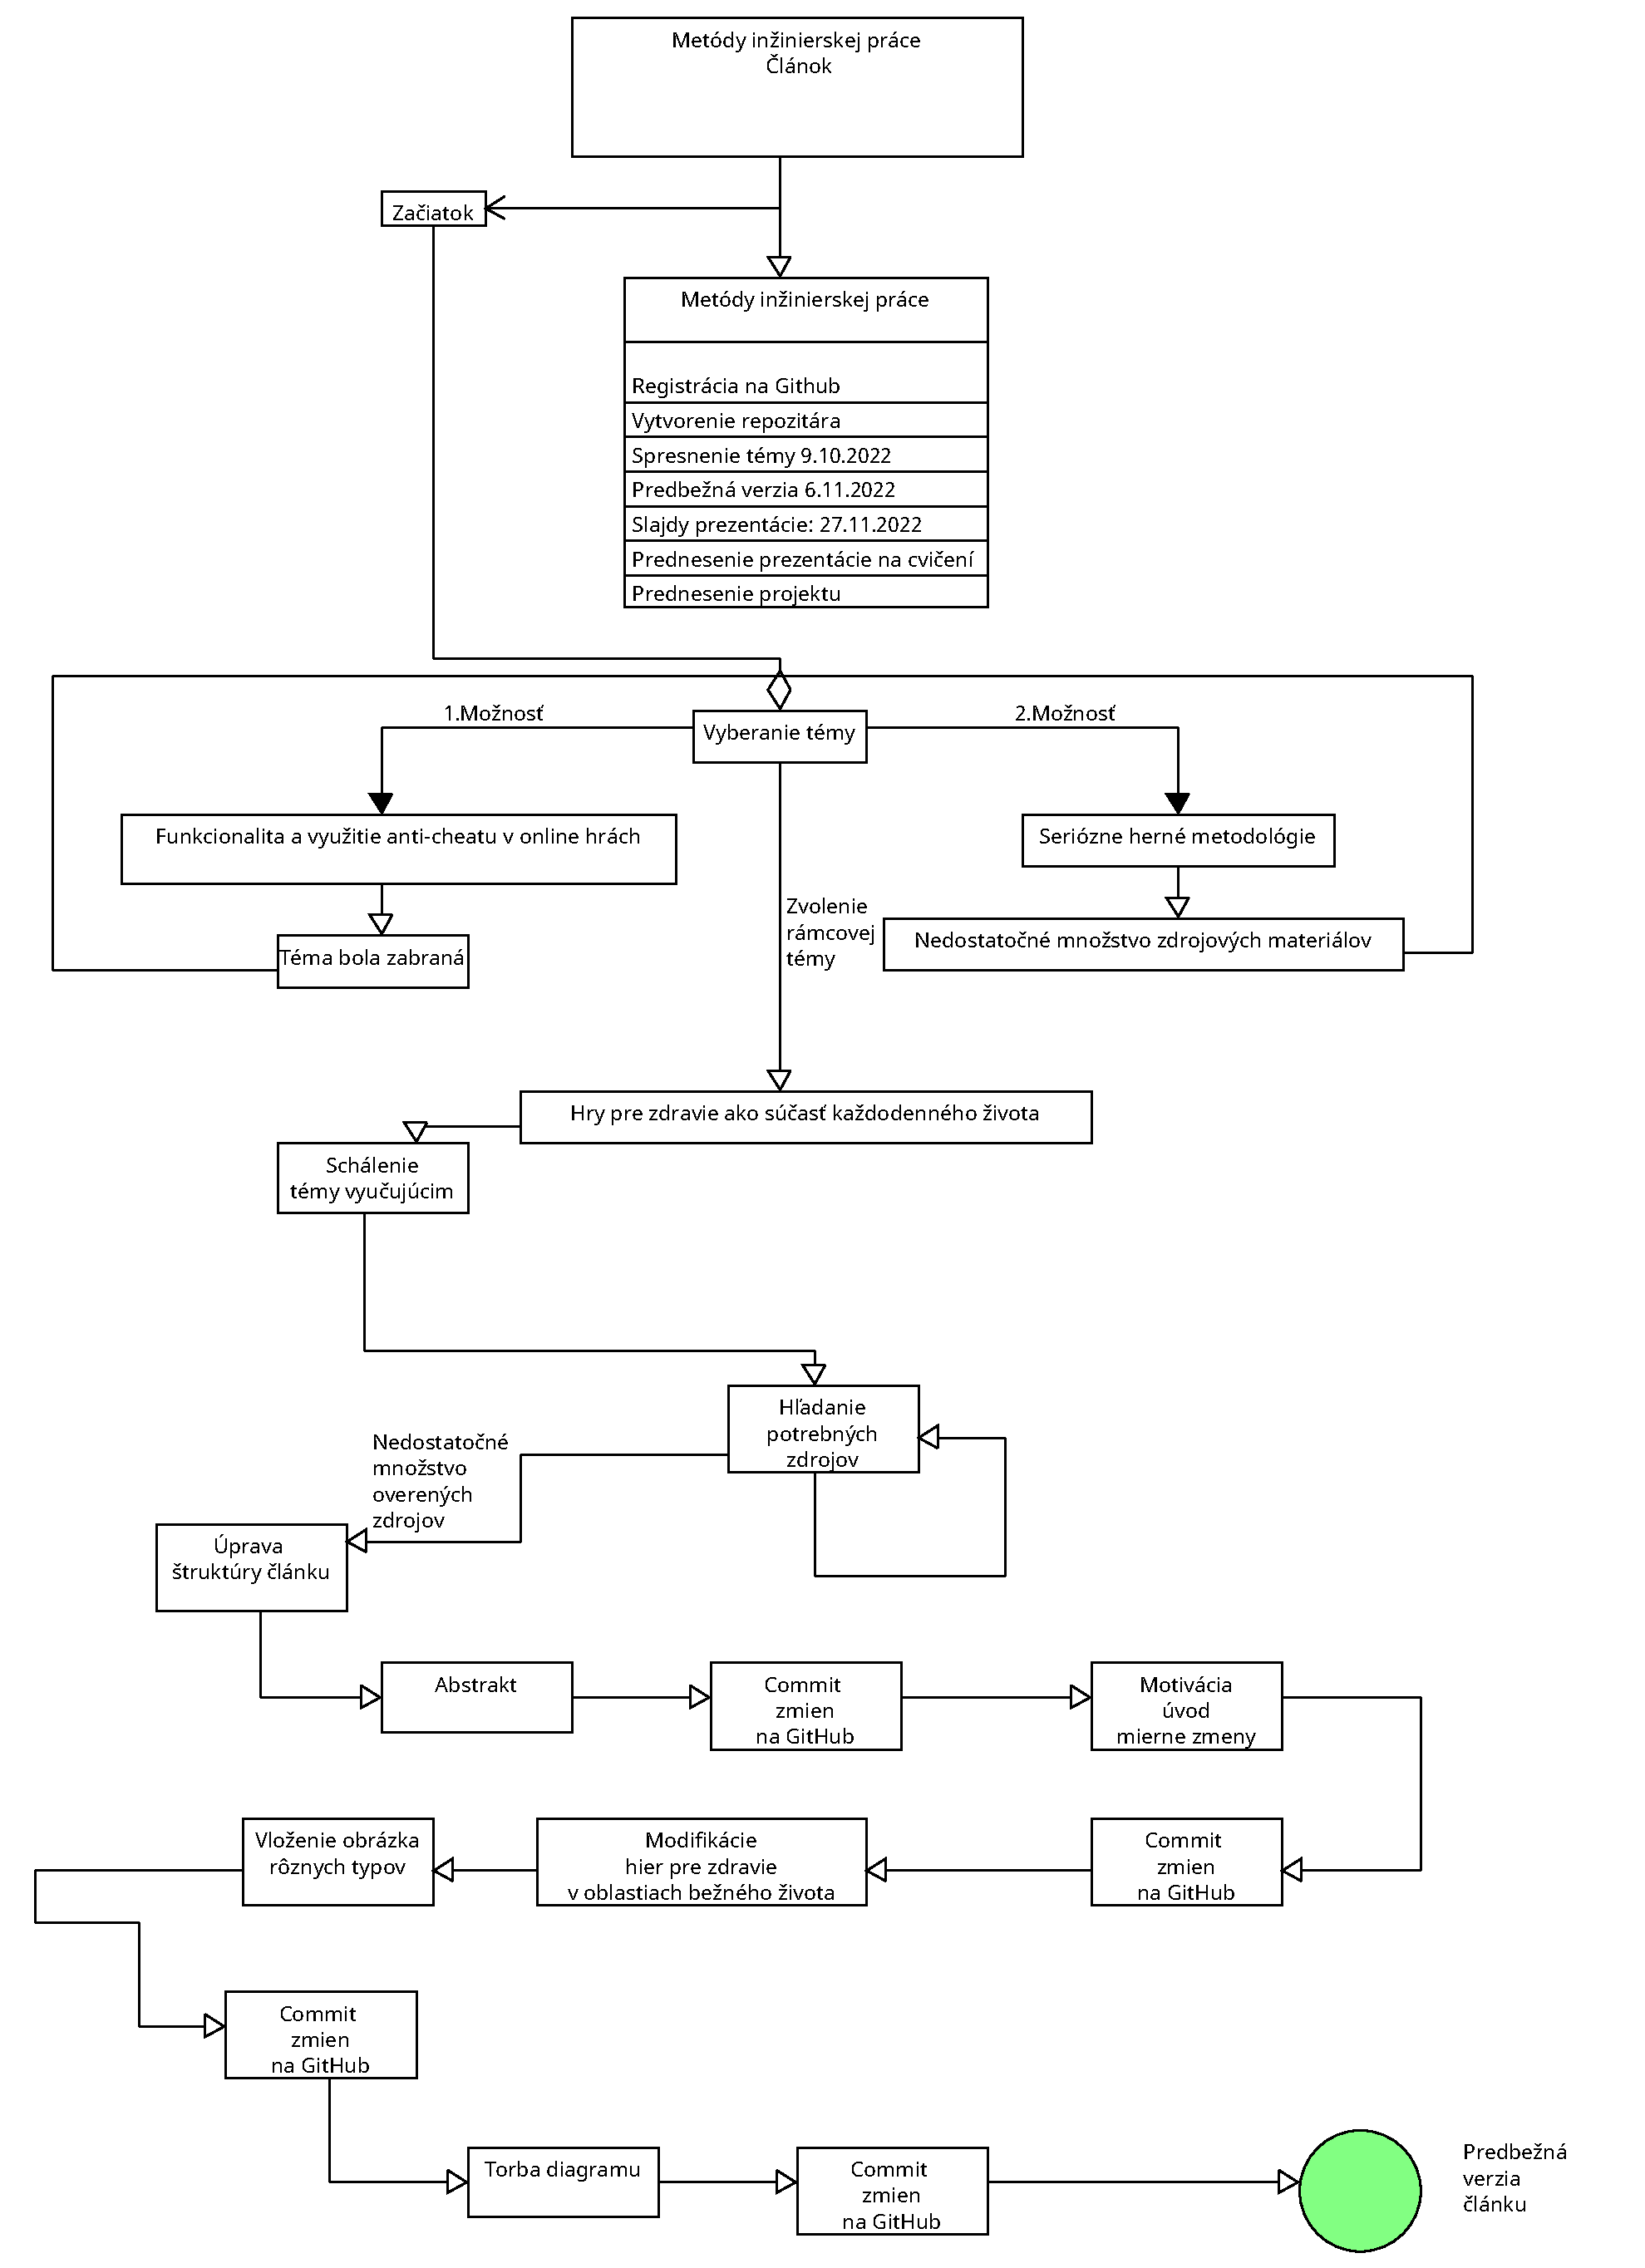
\includepdf[pages={1}]{Diagram_MIP.pdf}
\section{Proces zmien zapríčinený hrami pre zdravie}
Deti a dospievajúci sa častokrát učia počas hrania hir pomocou vizuálnej pozornosti.
\begin{figure*}[tbh]
\centering
%\includegraphics[scale=1.0]{diagram.pdf}
%Aj text môže byť prezentovaný ako obrázok. Stane sa z neho označný plávajúci objekt. Po vytvorení diagramu zrušte znak \texttt{\%} pred príkazom \verb|\includegraphics| označte tento riadok ako komentár (tiež pomocou znaku \texttt{\%}).
\caption{Kategórie hier.}
\label{f:rozhod}
\end{figure*}



%\section{Iná časť} \label{ina}

Základným problémom je teda\ldots{} Najprv sa pozrieme na nejaké vysvetlenie (časť~\ref{ina:nejake}), a potom na ešte nejaké %(časť~\ref{ina:nejake}).\footnote{Niekedy môžete potrebovať aj poznámku pod čiarou.}

Môže sa zdať, že problém vlastne nejestvuje, ale bolo dokázané, že to tak nie je~. Napriek tomu, aj dnes na webe narazíme na všelijaké pochybné názory. Dôležité veci možno \emph{zdôrazniť kurzívou}.


\subsection{Nejaké vysvetlenie} \label{ina:nejake}
\cite{Coplien:MPD}
Niekedy treba uviesť zoznam:

\begin{itemize}
\item jedna vec
\item druhá vec
	\begin{itemize}
	\item x
	\item y
	\end{itemize}
\end{itemize}

Ten istý zoznam, len číslovaný:

\begin{enumerate}
\item jedna vec
\item druhá vec
	\begin{enumerate}
	\item x
	\item y
	\end{enumerate}
\end{enumerate}


\subsection{Ešte nejaké vysvetlenie} \label{ina:este}

\paragraph{Veľmi dôležitá poznámka.}
Niekedy je potrebné nadpisom označiť odsek. Text pokračuje hneď za nadpisom.



\section{Dôležitá časť} \label{dolezita}





\section{Ešte dôležitejšia časť} \label{dolezitejsia}




\section{Záver} \label{zaver} % prípadne iný variant názvu



%\acknowledgement{Ak niekomu chcete poďakovať\ldots}


% týmto sa generuje zoznam literatúry z obsahu súboru literatura.bib podľa toho, na čo sa v článku odkazujete
\bibliography{literatura.bib}
\bibliographystyle{abbrv} % prípadne alpha, abbrv alebo hociktorý iný
\end{document}
